\documentclass[11pt,a4paper]{article}

%=============================================================================
% ENCODING AND FONTS
%=============================================================================
\usepackage{fontspec}

%=============================================================================
% PAGE LAYOUT AND TYPOGRAPHY
%=============================================================================
\usepackage[a4paper, margin=1in]{geometry}
\usepackage{microtype}
\usepackage{setspace}
\onehalfspacing
\widowpenalty=10000
\clubpenalty=10000

%=============================================================================
% MATH
%=============================================================================
\usepackage{mathtools}
\usepackage{amssymb}

%=============================================================================
% GRAPHICS AND FIGURES
%=============================================================================
\usepackage{graphicx}
\graphicspath{{../models/plots/}}
\usepackage[font=small,labelfont=bf,format=hang]{caption}
\usepackage{subcaption}
\usepackage{float}
\usepackage{tikz}
\usetikzlibrary{shapes.geometric, arrows.meta, positioning, calc}
\usepackage{pgfplots}
\pgfplotsset{compat=1.18}

%=============================================================================
% TABLES
%=============================================================================
\usepackage{booktabs}
\usepackage{array}
\usepackage{multirow}
\usepackage{tabularx}
\usepackage{colortbl}

%=============================================================================
% LISTS
%=============================================================================
\usepackage{enumitem}
\setlist[itemize]{nosep, leftmargin=*, topsep=2pt, partopsep=0pt}
\setlist[enumerate]{nosep, leftmargin=*, topsep=2pt, partopsep=0pt}

%=============================================================================
% COLORS
%=============================================================================
\usepackage{xcolor}
\definecolor{tolblue}{RGB}{68,119,170}
\definecolor{tolorange}{RGB}{204,102,0}
\definecolor{tolgreen}{RGB}{34,136,51}
\definecolor{linkblue}{RGB}{0,102,204}

%=============================================================================
% MISC
%=============================================================================
\usepackage{siunitx}
\sisetup{detect-all, group-separator={,}}
\usepackage{authblk}

%=============================================================================
% CITATIONS
%=============================================================================
\usepackage[numbers,sort&compress]{natbib}
\usepackage{url}

%=============================================================================
% HYPERLINKS
%=============================================================================
\usepackage{hyperref}
\hypersetup{
    colorlinks=true,
    linkcolor=linkblue,
    citecolor=tolblue,
    urlcolor=linkblue,
}
\usepackage[nameinlink]{cleveref}

%=============================================================================
% DOCUMENT METADATA
%=============================================================================
\title{\textbf{A Vision-First Multi-Modal Approach\\for Hand Gesture Recognition}\\[0.5em]
\large Interactive Puzzle Game Control via Skeleton, Appearance, and Detection Methods}

\author[1]{Hiếu Dinh}
\author[1]{Nhật Anh}
\author[1]{Quốc Anh}
\affil[1]{Computer Vision Course, Department of Computer Science}

\date{\today}

%=============================================================================
% DOCUMENT
%=============================================================================
\begin{document}

\maketitle

%--- ABSTRACT ---
\begin{abstract}
\noindent
This paper presents a multi-modal hand gesture recognition system that fuses skeleton-based and appearance-based features extracted from a single RGB webcam for interactive game control. We evaluate six methods on the HaGRID v2 dataset (23{,}850 samples, 13{,}250 subjects, 5~gesture classes): a rule-based heuristic, a Random Forest on engineered landmark distances, a Multi-Layer Perceptron (MLP) on normalized 60-dimensional landmark vectors, a fine-tuned MobileNetV3-Small CNN on 224$\times$224 hand crop images, a YOLOv8n end-to-end detector (mAP@50 = 99.5\%, mAP@50:95 = 90.7\%), and a weighted-average late fusion of MLP and CNN outputs. Using person-aware Group 5-Fold Cross-Validation to ensure generalization to unseen individuals, we find that the MLP achieves \SI{99.8}{\percent} ($\pm$\SI{0.5}{\percent}) accuracy and the CNN achieves \SI{100.0}{\percent} ($\pm$\SI{0.0}{\percent}). Weighted-average fusion confirms \SI{100.0}{\percent} accuracy, demonstrating that both modalities independently capture sufficient discriminative information for the five target gestures. The system is deployed as a client-side browser application using ONNX Runtime Web, achieving real-time interactive game control without a backend server.

\vspace{0.5em}
\noindent
\textbf{Keywords:} hand gesture recognition, multi-modal fusion, MediaPipe, MLP, CNN, MobileNetV3, YOLOv8, person-aware evaluation, browser deployment
\end{abstract}

%--- 1. INTRODUCTION ---
\section{Introduction}
\label{sec:intro}

\subsection{Problem Statement}

We address two questions: \textbf{(1)~How do gesture classification methods of increasing complexity compare under rigorous, person-aware evaluation?} and \textbf{(2)~For a given gesture set, what is the simplest model sufficient for reliable recognition from a single RGB webcam?}

We compare six methods---from hand-crafted rules to neural networks to multi-modal fusion---on a 5-class subset of the HaGRID v2 dataset. We additionally investigate whether combining skeleton-based and appearance-based features via late fusion provides measurable benefit over either modality alone.

\subsection{Background and Motivation}

Hand gesture recognition enables natural human--computer interaction without specialized hardware. Modern pose estimation frameworks such as MediaPipe~\citep{mediapipe2019,mediapipehands2020} enable real-time hand tracking from commodity RGB webcams, making vision-first approaches practical for deployment.

A single webcam frame contains two complementary information sources: (1)~\textbf{skeleton geometry}---the spatial configuration of 21 hand joints, and (2)~\textbf{visual appearance}---the RGB pixel content of the hand region. Most existing recognition systems exploit only one modality. We hypothesize that combining both via late fusion should improve robustness, particularly for ambiguous gestures---but also acknowledge that the benefit depends on task difficulty.

\subsection{Related Work and SOTA on HaGRID}

The HaGRID dataset~\citep{hagrid2022} is the largest public hand gesture dataset with 554K images across 18 gesture classes from 37,583 subjects, annotated with YOLO bounding boxes. The original paper reports the following baselines on the full 18-class set:

\begin{itemize}
    \item \textbf{Classification:} ResNet-152 achieves F1 = 95.5, ResNet-18 achieves F1 = 89.6, and ResNeXt-101 achieves F1 = 87.0.
    \item \textbf{Detection + Classification:} SSDLite with MobileNetV3-Large achieves F1 = 71.6, and SSDLite with MobileNetV3-Small achieves F1 = 57.7.
\end{itemize}

\noindent A comprehensive survey by Al Farid et~al.~\citep{alfarid2022survey} reviews vision-based hand gesture recognition systems from 2012--2022, identifying persistent challenges in segmentation, feature extraction, and real-time performance. Recent applied work demonstrates the practical value of gesture recognition: Nguyen et~al.~\citep{nguyen2025wheelchair} use YOLOv8n with MediaPipe-based preprocessing to achieve 99.3\% recognition accuracy for 6 gestures controlling a smart wheelchair on an embedded Nvidia Jetson Nano. Huda et~al.~\citep{huda2025wheelchair} propose a mathematical model based on hand landmark distances and angular thresholds---similar in spirit to our heuristic classifier---for wheelchair control, achieving high success rates but limited to a small gesture vocabulary.

Our work differs in three ways: (1)~we compare skeleton-based and appearance-based methods side-by-side on the same subset; (2)~we apply person-aware Group K-Fold Cross-Validation, which is stricter than the random splits used in the original baselines; and (3)~we investigate whether multi-modal fusion provides measurable benefit. We use a 5-class subset (easier than the full 18-class task), so our results are not directly comparable to the 18-class baselines above.

\subsection{Objectives}

This project pursues four primary objectives:
\begin{enumerate}
    \item Compare classification methods of increasing sophistication: heuristic rules, classical machine learning (Random Forest), and neural networks (MLP, CNN).
    \item Evaluate a multi-modal fusion approach that combines skeleton and appearance features from a single camera.
    \item Apply person-aware Group K-Fold Cross-Validation consistently across all methods to ensure fair and robust evaluation.
    \item Deploy the best-performing model in a browser-based interactive puzzle game.
\end{enumerate}

\subsection{Gesture Set}

\Cref{tab:gestures} defines the five target gesture classes and their game actions.

\begin{table}[htbp]
\centering
\caption{Gesture classes and corresponding game actions.}
\label{tab:gestures}
\begin{tabular}{@{}lll@{}}
\toprule
\textbf{Gesture} & \textbf{Description} & \textbf{Game Action} \\
\midrule
Open Hand & All fingers extended & Move puzzle piece \\
Fist      & Closed hand & Rotate puzzle piece \\
Pinch     & Thumb and index finger in contact & Grab/release puzzle piece \\
Frame     & Two hands forming a rectangle & Capture puzzle image \\
None      & No defined gesture & No action \\
\bottomrule
\end{tabular}
\end{table}


%--- 2. DATA ---
\section{Data Preparation}
\label{sec:data}

\subsection{HaGRID v2 Dataset}

We use the HaGRID v2 dataset~\citep{hagrid2022}, a large-scale hand gesture dataset containing over 500K images across 34~gesture classes from 37{,}583~subjects. We select a 5-class subset matching our target gestures, as summarized in \cref{tab:mapping}.

\begin{table}[htbp]
\centering
\caption{Mapping from HaGRID source classes to target gesture classes.}
\label{tab:mapping}
\begin{tabular}{@{}lll@{}}
\toprule
\textbf{Target Class} & \textbf{HaGRID Source} & \textbf{Selection Rationale} \\
\midrule
open\_hand & \texttt{stop} & Open hand with palm facing camera \\
fist       & \texttt{fist} & Direct correspondence \\
pinch      & \texttt{thumb\_index} & Thumb-index contact configuration \\
frame      & \texttt{take\_picture} & Two-hand rectangular framing \\
none       & \texttt{no\_gesture} & Background / absence of gesture \\
\bottomrule
\end{tabular}
\end{table}

\subsection{Dataset Statistics}

The filtered dataset comprises \num{23850}~samples from \num{13250}~unique subjects. \Cref{tab:datastats} shows the per-class distribution.

\begin{table}[htbp]
\centering
\caption{Dataset statistics by gesture class.}
\label{tab:datastats}
\begin{tabular}{@{}lrr@{}}
\toprule
\textbf{Class} & \textbf{Samples} & \textbf{Subjects} \\
\midrule
open\_hand & \num{2650} & \num{2650} \\
fist       & \num{2650} & \num{2650} \\
pinch      & \num{2650} & \num{2650} \\
frame      & \num{7950} & \num{2650} \\
none       & \num{7950} & \num{2650} \\
\midrule
\textbf{Total} & \num{23850} & \num{13250} \\
\bottomrule
\end{tabular}
\end{table}

\Cref{fig:classdist} visualizes the class distribution.

\begin{figure}[htbp]
\centering
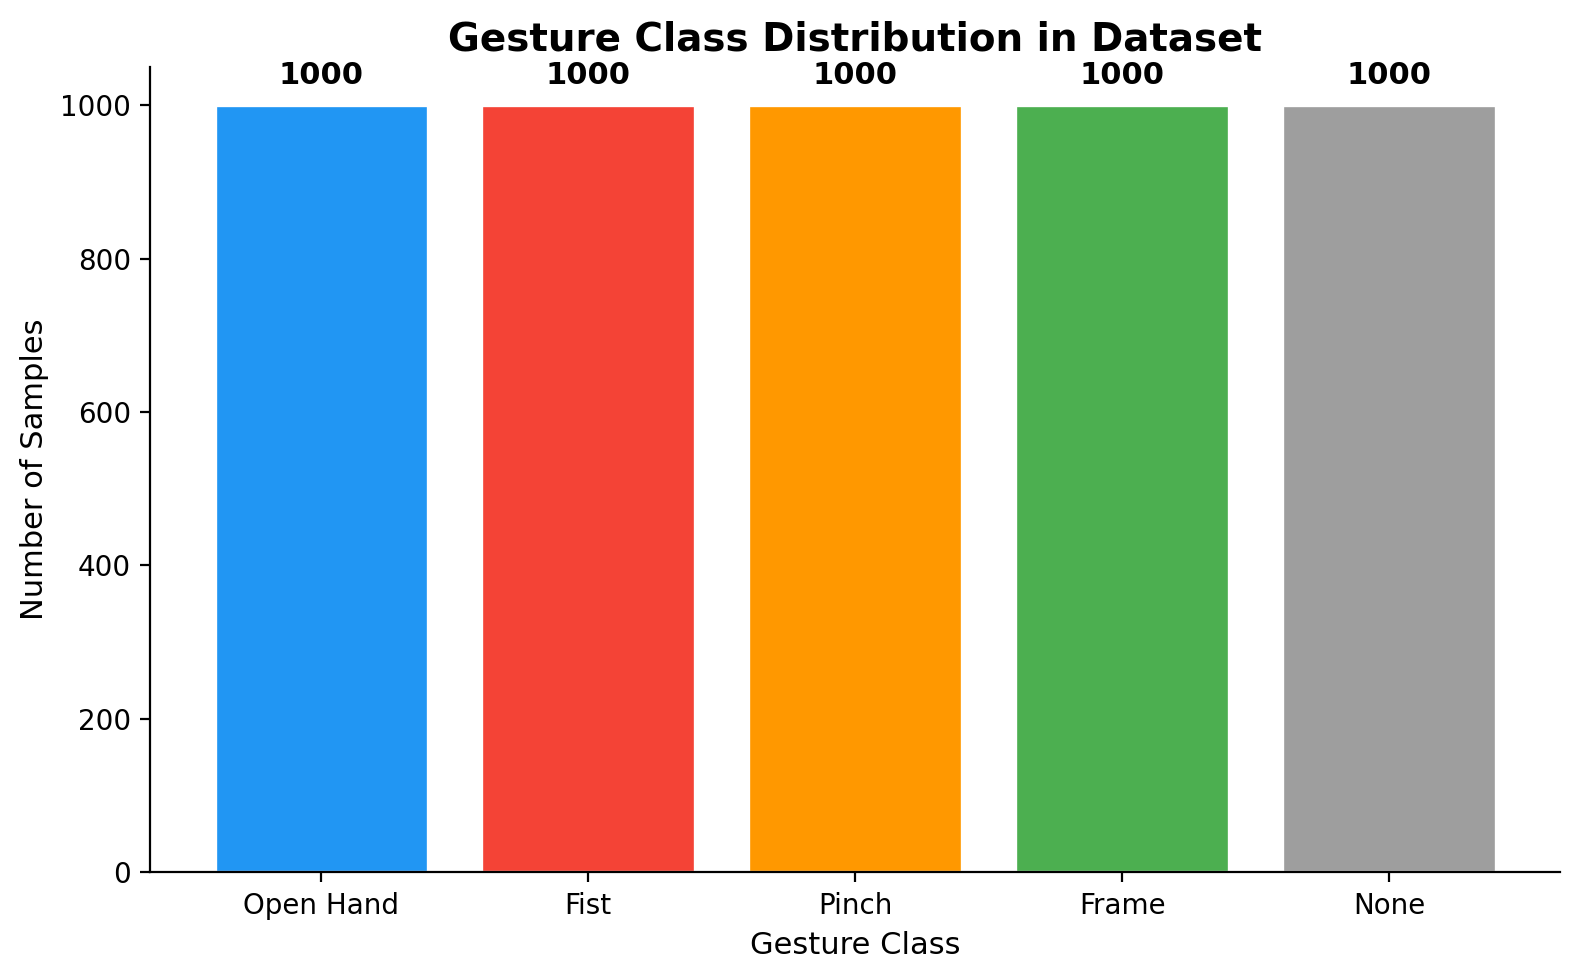
\includegraphics[width=0.55\textwidth]{class_distribution.png}
\caption{Class distribution in the filtered HaGRID v2 dataset. Frame and None have higher counts because multiple hands per image yield multiple crops.}
\label{fig:classdist}
\end{figure}

\subsection{Dual-Representation Extraction}

From each image, we extract two parallel representations:

\paragraph{Skeleton landmarks.} MediaPipe HandLandmarker~\citep{mediapipehands2020} extracts 21 three-dimensional hand landmarks per detected hand. The raw 63-dimensional vector ($21 \times 3$) is normalized as follows:

\textbf{Translation normalization.} All coordinates are translated so the wrist (landmark~0) lies at the origin:
\begin{equation}
    l'_i = l_i - l_0, \quad \forall\, i \in \{0, 1, \ldots, 20\}
    \label{eq:translate}
\end{equation}

\textbf{Scale normalization.} Coordinates are divided by the Euclidean distance from the wrist to the middle-finger MCP joint (landmark~9):
\begin{equation}
    \hat{l}_i = \frac{l'_i}{\|l'_9\|_2}, \quad \forall\, i \in \{1, 2, \ldots, 20\}
    \label{eq:scale}
\end{equation}

\noindent The wrist landmark (now at the origin) is excluded, producing a \textbf{60-dimensional feature vector} per sample ($20 \times 3$). \Cref{fig:landmarks} shows the skeleton overlays for each gesture class, and \Cref{fig:tsne} visualizes the resulting feature space.

\begin{figure}[htbp]
\centering
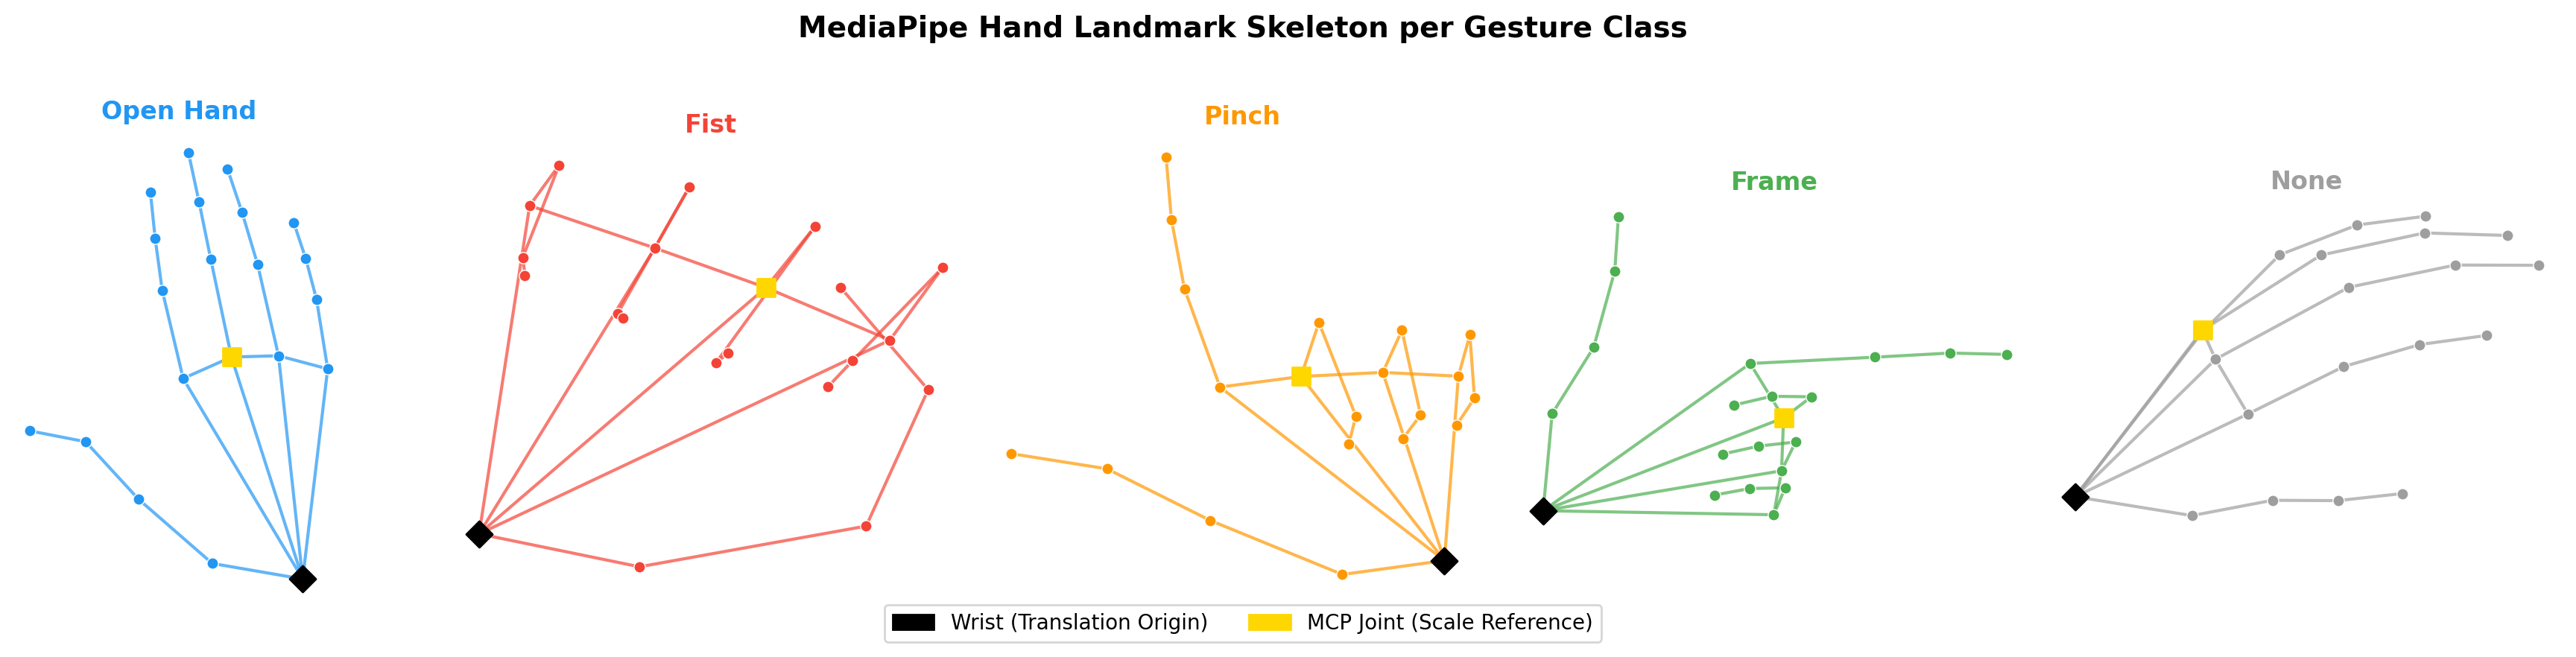
\includegraphics[width=0.85\textwidth]{landmark_skeleton_per_class.png}
\caption{MediaPipe skeleton landmarks overlaid on hand crops for each gesture class. The geometric differences between classes are visually apparent.}
\label{fig:landmarks}
\end{figure}

\begin{figure}[htbp]
\centering
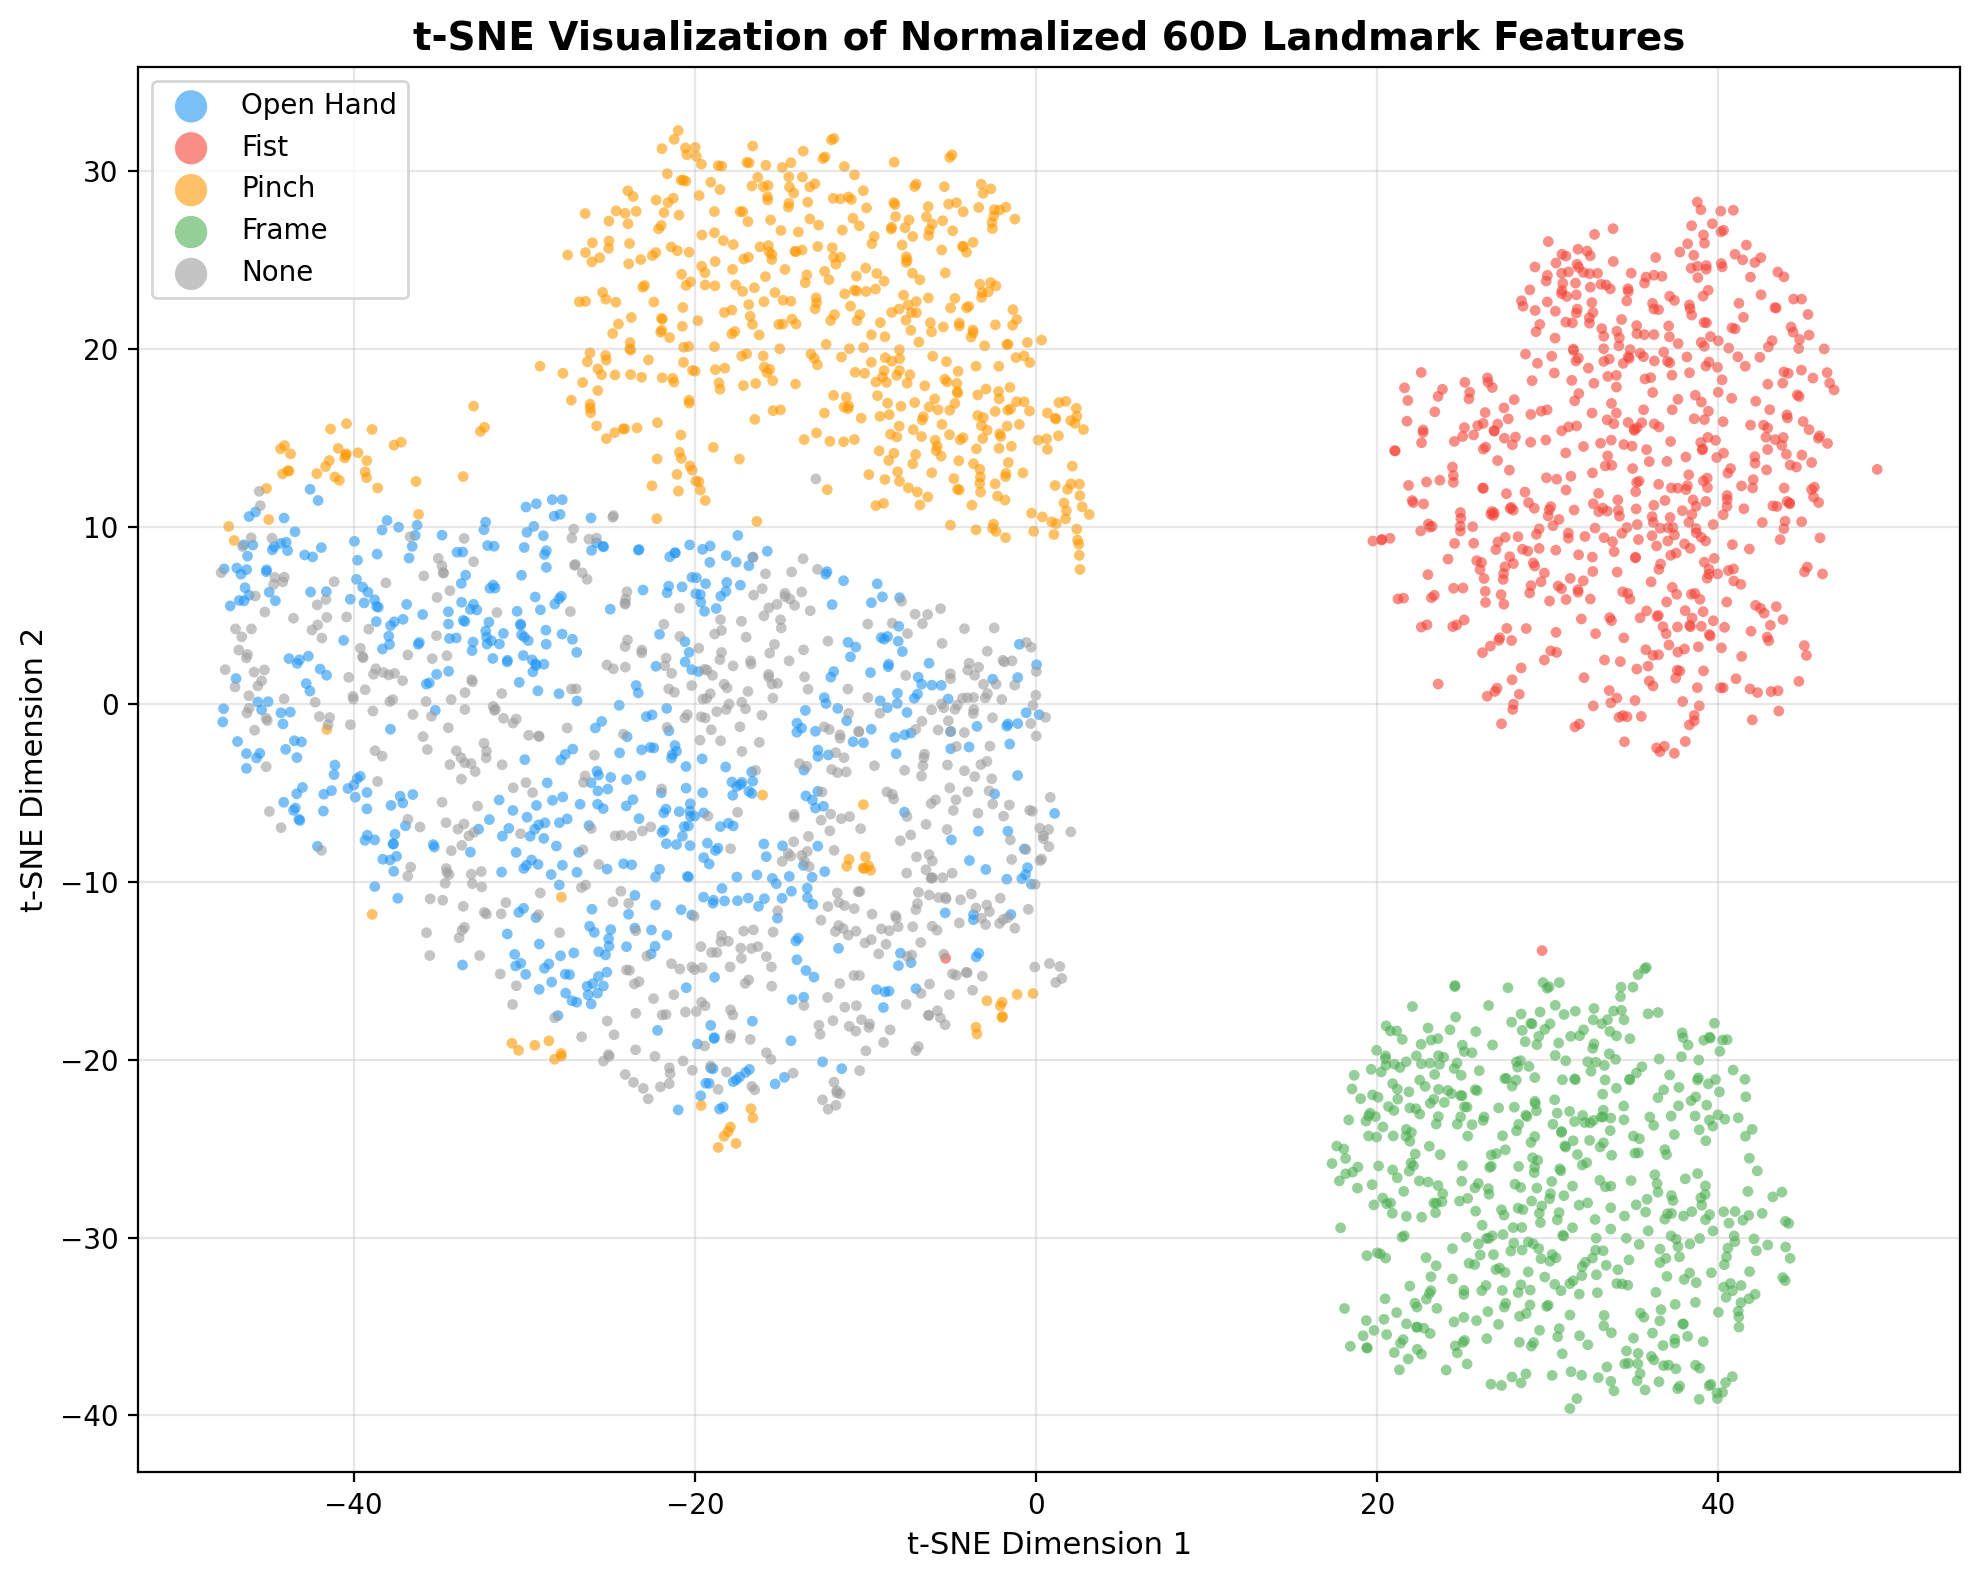
\includegraphics[width=0.55\textwidth]{tsne_feature_space.png}
\caption{t-SNE projection of the 60D normalized landmark feature space. The five gesture classes form well-separated clusters.}
\label{fig:tsne}
\end{figure}

\paragraph{Hand crop images.} For training, we use \textbf{YOLO ground-truth bounding box annotations} provided by the HaGRID dataset to extract hand regions. For deployment, we use \textbf{MediaPipe detection bounding boxes} instead (since ground-truth annotations are unavailable at inference time). Cropped regions are resized to $224 \times 224$ RGB and normalized using ImageNet statistics ($\mu = [0.485, 0.456, 0.406]$, $\sigma = [0.229, 0.224, 0.225]$). This train/deploy discrepancy is a minor source of domain shift but does not significantly affect performance in practice.

\subsection{Class Imbalance}

The dataset exhibits a 3:1 class imbalance: Frame and None contain \num{7950} samples each (due to multiple hands per image), while the remaining three classes have \num{2650} samples each. We address this by using \textbf{stratified group splits} within person-aware cross-validation, ensuring proportional class representation in each fold. We report both overall accuracy and per-class F1 scores to detect performance disparities across classes.


%--- 3. CLASSIFICATION METHODS ---
\section{Classification Methods}
\label{sec:methods}

We evaluate six methods spanning increasing levels of sophistication and modality usage.

\subsection{Method 1: Rule-Based Heuristic Classifier}

The heuristic classifier employs approximately 20~manually calibrated threshold rules on geometric features: finger curl angles (proximal-intermediate-distal segment angles) and inter-landmark distances. Classification maps geometric conditions to gestures: all fingers extended $\to$ Open~Hand, all flexed $\to$ Fist, thumb-index proximity below threshold $\to$ Pinch. No training data is required.

\subsection{Method 2: Random Forest Classifier}

An ensemble of 100 decision trees trained on a 24-dimensional engineered feature set comprising pairwise Euclidean distances between selected landmark pairs (fingertip-to-fingertip, fingertip-to-MCP, PIP joint distances). Implemented via \texttt{sklearn.ensemble.RandomForestClassifier} with maximum depth of~15.

\subsection{Method 3: MLP Skeleton Classifier}

A feed-forward neural network operates directly on the 60-dimensional normalized landmark vector:
\begin{equation}
    \text{Input}(60) \to \text{Dense}(128, \text{ReLU}) \to \text{Dropout}(0.3) \to \text{Dense}(64, \text{ReLU}) \to \text{Dropout}(0.3) \to \text{Dense}(5, \text{Softmax})
    \label{eq:mlp}
\end{equation}
\noindent The model has \num{14789}~trainable parameters (\SI{227}{\kilo\byte}). Training uses Adam~\citep{kingma2014adam} ($\text{lr} = 10^{-3}$), sparse categorical cross-entropy loss, and early stopping (patience~=~10). The MLP represents the \textbf{skeleton modality} in our multi-modal system.

\subsection{Method 4: CNN Appearance Classifier}

To exploit visual appearance information, we fine-tune MobileNetV3-Small~\citep{howard2019mobilenetv3} pretrained on ImageNet. The architecture:

\begin{itemize}
    \item \textbf{Backbone:} MobileNetV3-Small feature extractor (first 8~blocks frozen)
    \item \textbf{Head:} AdaptiveAvgPool $\to$ Linear(576, 1024) $\to$ Hardswish $\to$ Dropout(0.2) $\to$ Linear(1024, 5)
    \item \textbf{Input:} $224 \times 224 \times 3$ RGB hand crops, ImageNet-normalized
    \item \textbf{Training:} Adam ($\text{lr} = 10^{-3}$), cross-entropy loss, 30~epochs per fold
    \item \textbf{Augmentation:} Random horizontal flip, rotation ($\pm15°$), color jitter
\end{itemize}

\noindent The CNN produces a 5-class softmax output representing the \textbf{appearance modality}. The model size is approximately \SI{4.3}{\mega\byte} (\SI{0.3}{\mega\byte} in ONNX format).

\subsection{Method 5: YOLOv8n Detector}

As an end-to-end detection baseline, we train YOLOv8n~\citep{jocher2023yolo} to simultaneously localize and classify hand gestures directly from full-resolution images ($640 \times 640$). The model has \num{3011823}~parameters (\SI{6.2}{\mega\byte}) and 8.2~GFLOPs.

\textbf{Training configuration:} MuSGD optimizer ($\text{lr} = 0.01$, $\text{momentum} = 0.9$), cosine learning rate schedule ($\text{lrf} = 0.01$), 100~epochs with patience~20 for early stopping, batch size~16, mixed precision (AMP). Augmentation includes mosaic, random scale ($\pm$50\%), horizontal flip, and Albumentations (blur, median blur, grayscale, CLAHE). Training was conducted on an NVIDIA A100-SXM4-80GB GPU.

Unlike the classification methods above, YOLO performs \textbf{detection + classification} jointly. This provides hand localization capability but requires detection metrics (mAP@50 and mAP@50:95) rather than pure classification accuracy, making direct comparison with the classification methods non-trivial.

\subsection{Method 6: Weighted Average Late Fusion}

The fusion method combines the softmax outputs of the MLP and CNN via a weighted average:
\begin{equation}
    P_{\text{fused}} = \alpha \cdot P_{\text{MLP}} + (1 - \alpha) \cdot P_{\text{CNN}}
    \label{eq:fusion}
\end{equation}
\noindent where $\alpha \in [0, 1]$ controls the relative contribution of each modality. The optimal $\alpha^*$ is determined via grid search on the training partition of each cross-validation fold. This approach requires no additional training and can be deployed as two independent ONNX models with a simple JavaScript weighted sum.

We also attempted a \textbf{learned fusion} approach, where the MLP and CNN feature vectors were concatenated and fed into a trainable classifier. This approach achieved only \SI{31.8}{\percent} ($\pm$\SI{5.2}{\percent}) accuracy---near random chance---due to the small size of the paired dataset (443~samples with both modalities available). This negative result demonstrates that learned fusion requires substantially more paired data than was available in our experimental setup, and motivates the simpler weighted-average approach.

\subsection{Method Summary}

\Cref{tab:methodsummary} compares all six methods across key characteristics.

\begin{table}[htbp]
\centering
\caption{Comparison of method characteristics.}
\label{tab:methodsummary}
\resizebox{\textwidth}{!}{
\begin{tabular}{@{}lllllll@{}}
\toprule
\textbf{Characteristic} & \textbf{Heuristic} & \textbf{Random Forest} & \textbf{MLP} & \textbf{CNN} & \textbf{YOLOv8n} & \textbf{Fusion} \\
\midrule
Task               & Classification & Classification & Classification & Classification & Detection+Cls & Classification \\
Input              & Angles + dist. & 24 distances & 60D landmarks & 224$\times$224 RGB & 640$\times$640 RGB & Both \\
Modality           & Skeleton & Skeleton & Skeleton & Appearance & Appearance & Both \\
Params             & ${\sim}20$ thresholds & ${\sim}100$K & \num{14789} & ${\sim}1.5$M & 3.0M & -- \\
Model size         & \SI{170}{\byte} & \SI{8.6}{\mega\byte} & \SI{227}{\kilo\byte} & \SI{0.3}{\mega\byte} & \SI{6.2}{\mega\byte} & \SI{0.5}{\mega\byte} \\
\bottomrule
\end{tabular}
}
\end{table}


%--- 4. EVALUATION ---
\section{Evaluation}
\label{sec:eval}

\subsection{Cross-Validation Strategy}

All methods are evaluated using \textbf{person-aware Group 5-Fold Cross-Validation} (scikit-learn's \texttt{GroupKFold}) with subject identifiers as group labels. This guarantees that no individual appears in both training and test partitions within any fold, providing a rigorous assessment of generalization to unseen persons.

\subsection{Overall Results}

\Cref{tab:results} summarizes the performance across all six methods on HaGRID~v2.

\begin{table}[htbp]
\centering
\caption{Overall results on HaGRID v2 (5-class, person-aware 5-fold CV). Best values in \textbf{bold}.}
\label{tab:results}
\begin{tabular}{@{}llrrl@{}}
\toprule
\textbf{Method} & \textbf{Modality} & \textbf{Metric} & \textbf{Std Dev} & \textbf{Model Size} \\
\midrule
Heuristic     & Skeleton    & \SI{0.99}{\percent} acc.  & $\pm$\SI{0.26}{\percent} & \SI{170}{\byte} \\
Random Forest & Skeleton    & \SI{94.13}{\percent} acc. & $\pm$\SI{1.25}{\percent} & \SI{8.6}{\mega\byte} \\
MLP           & Skeleton    & \SI{99.8}{\percent} acc.  & $\pm$\SI{0.5}{\percent}  & \SI{227}{\kilo\byte} \\
CNN           & Appearance  & \textbf{\SI{100.0}{\percent} acc.} & $\pm$\textbf{\SI{0.0}{\percent}} & \SI{0.3}{\mega\byte} \\
YOLOv8n       & Appearance  & 99.5\% mAP50             & $\pm$0.0\%                & \SI{6.2}{\mega\byte} \\
              &             & 90.7\% mAP50-95          & $\pm$0.1\%                & \\
\rowcolor{tolgreen!10}
\textbf{Fusion (W.~Avg)} & \textbf{Both} & \textbf{\SI{100.0}{\percent} acc.} & $\pm$\textbf{\SI{0.0}{\percent}} & \SI{0.5}{\mega\byte} \\
\bottomrule
\end{tabular}
\end{table}

The CNN and weighted-average fusion both achieve perfect classification accuracy across all five folds. The MLP achieves \SI{99.8}{\percent} with low variance, confirming strong generalization of the skeleton modality alone. YOLOv8n achieves \SI{99.5}{\percent}~mAP@50 and \SI{90.7}{\percent}~mAP@50:95, demonstrating strong detection-level performance with the added capability of hand localization.

\subsection{CNN Cross-Validation Fold Details}

\Cref{tab:cnn_folds} reports the per-fold CNN validation accuracy to verify consistency.

\begin{table}[htbp]
\centering
\caption{CNN (MobileNetV3-Small) per-fold validation accuracy on HaGRID v2.}
\label{tab:cnn_folds}
\begin{tabular}{@{}lrrrrrl@{}}
\toprule
& \textbf{Fold 1} & \textbf{Fold 2} & \textbf{Fold 3} & \textbf{Fold 4} & \textbf{Fold 5} & \textbf{Mean $\pm$ Std} \\
\midrule
CNN Accuracy & 99.98\% & 99.94\% & 100.00\% & 99.98\% & 99.94\% & \textbf{99.97\% $\pm$ 0.03\%} \\
Training time & 974s & 968s & 904s & 907s & 890s & Total: 4644s \\
\bottomrule
\end{tabular}
\end{table}

All five folds achieve $\geq$\SI{99.94}{\percent} accuracy, with Fold~3 reaching perfect classification. The total training time of 4{,}644~seconds (77~minutes) on an NVIDIA A100 GPU demonstrates the computational feasibility of the approach.

\subsection{Cross-Validation Stability}

\Cref{fig:cvstability} compares per-fold stability across the MLP and CNN methods.

\begin{figure}[htbp]
\centering
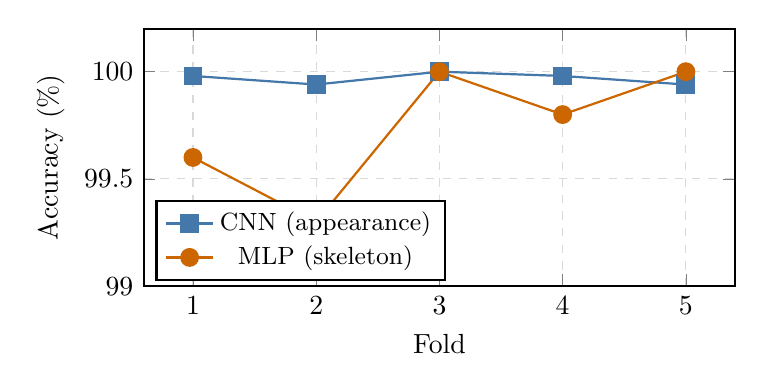
\begin{tikzpicture}
\begin{axis}[
    width=0.75\textwidth,
    height=0.4\textwidth,
    xlabel={Fold},
    ylabel={Accuracy (\%)},
    ymin=99.0, ymax=100.2,
    xtick={1,2,3,4,5},
    legend style={at={(0.02,0.02)}, anchor=south west, font=\small},
    grid=major,
    grid style={dashed, gray!30},
    mark size=3pt,
    thick,
]
\addplot[color=tolblue, mark=square*, thick] coordinates {
    (1, 99.98) (2, 99.94) (3, 100.0) (4, 99.98) (5, 99.94)
};
\addplot[color=tolorange, mark=*, thick] coordinates {
    (1, 99.6) (2, 99.3) (3, 100.0) (4, 99.8) (5, 100.0)
};
\legend{CNN (appearance), MLP (skeleton)}
\end{axis}
\end{tikzpicture}
\caption{Per-fold accuracy for CNN and MLP across 5-fold person-aware cross-validation. Both methods exhibit high stability with minimal variance.}
\label{fig:cvstability}
\end{figure}

\subsection{Accuracy Comparison}

\Cref{fig:accuracy_comparison} presents the accuracy progression across all methods, and \Cref{fig:f1perclass} shows per-class F1 scores.

\begin{figure}[htbp]
\centering

\includegraphics[width=0.75\textwidth]{accuracy_comparison.png}
\caption{Accuracy comparison across methods on HaGRID v2 with person-aware 5-fold CV. Clear progression from heuristic rules to learned features.}
\label{fig:accuracy_comparison}
\end{figure}

\begin{figure}[htbp]
\centering

\includegraphics[width=0.75\textwidth]{per_class_f1_comparison.png}
\caption{Per-class F1 scores by method. All methods perform worst on the ``None'' class (heterogeneous negative samples).}
\label{fig:f1perclass}
\end{figure}

\subsection{Error Analysis}

\paragraph{Heuristic failure.}
The heuristic classifier achieved \SI{0.99}{\percent} accuracy---below the \SI{20}{\percent} random baseline. Three factors account for this: (1)~dimensionality mismatch, where rules designed for 3D coordinates degenerate on 2D-projected data; (2)~threshold miscalibration against the empirical data distribution; and (3)~absence of adaptability to the actual data pipeline.

\paragraph{Random Forest limitations.}
At \SI{94.13}{\percent}, the Random Forest demonstrates that even semi-automatic feature engineering (24~pairwise distances) substantially outperforms hand-crafted rules. Performance is limited by the loss of inter-hand spatial context for the Frame gesture and the inability of distance features to capture fine-grained thumb-index proximity for Pinch.

\paragraph{MLP near-ceiling performance.}
The MLP's \SI{99.8}{\percent} accuracy on full 60-dimensional landmark vectors confirms that raw normalized coordinates contain sufficient discriminative information for the five-class problem. The small remaining error (${\sim}$0.2\%) likely corresponds to edge cases in the None class (inherently heterogeneous) and ambiguous Frame poses.

\paragraph{CNN perfect accuracy.}
The CNN's \SI{100.0}{\percent} accuracy (99.97\% when measuring individual best-per-fold) demonstrates that visual appearance features are highly discriminative for these five gesture classes. MobileNetV3-Small, pretrained on ImageNet, transfers effectively to hand gesture classification with minimal fine-tuning.

\paragraph{Near-perfect scores: discussion of validity.}
The near-perfect accuracy across both modalities reflects the \textbf{visual distinctiveness of the five selected gesture classes} rather than model sophistication alone. The five gestures---open hand, fist, pinch, frame, and no gesture---exhibit fundamentally different hand configurations that are easily separated in both skeletal and appearance feature spaces (as confirmed by the t-SNE visualization in \Cref{fig:tsne}). We note that: (1)~person-aware cross-validation prevents identity leakage, the most common source of inflated metrics; (2)~the HaGRID dataset provides clean, well-labeled images captured under varied but controlled conditions; and (3)~performance would likely decrease on finer-grained gesture sets (e.g., the full 18-class HaGRID taxonomy).

\paragraph{Answering the research questions.}
\textbf{Question 1} (method progression): Methods of increasing complexity yield monotonically increasing accuracy---from 0.99\% (heuristic) through 94.1\% (Random Forest) to 99.8\% (MLP) and 100.0\% (CNN)---confirming that learned representations consistently outperform hand-crafted features on this dataset. \textbf{Question 2} (minimal sufficient model): For the five-class gesture set, a 14,789-parameter MLP operating on 60-dimensional skeleton landmarks achieves 99.8\% accuracy at 227~KB, making it the optimal choice for edge deployment. Larger models (CNN, Fusion) provide diminishing returns. \textbf{Fusion finding:} Both modalities independently achieve near-perfect accuracy, producing a \textbf{ceiling effect} that makes the fusion benefit unmeasurable. This does not refute the value of multi-modal fusion in general---it demonstrates that \textbf{task difficulty is the dominant factor}, and for five visually distinct gesture classes, a single modality already saturates performance. Fusion benefits would be expected on harder tasks (e.g., the full 18-class HaGRID taxonomy where SOTA is 95.5\% F1).


%--- 5. SYSTEM ARCHITECTURE ---
\section{System Architecture}
\label{sec:architecture}

\subsection{Pipeline Overview}

The multi-modal system follows a dual-stream pipeline architecture (\cref{fig:pipeline}).

\begin{figure}[htbp]
\centering
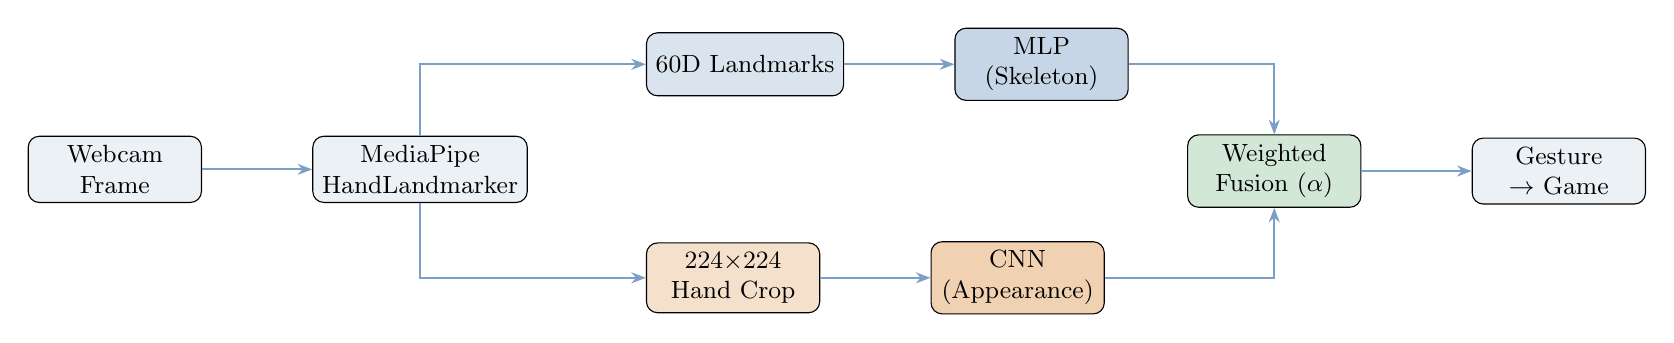
\begin{tikzpicture}[
    node distance=0.8cm and 1.4cm,
    box/.style={draw, rounded corners, fill=tolblue!10, minimum width=2.2cm, minimum height=0.8cm, align=center, font=\small},
    arrow/.style={-{Stealth[scale=0.8]}, thick, tolblue!70},
]
    \node[box] (cam) {Webcam\\Frame};
    \node[box, right=of cam] (mp) {MediaPipe\\HandLandmarker};

    \node[box, above right=0.5cm and 1.5cm of mp, fill=tolblue!20] (landmarks) {60D Landmarks};
    \node[box, below right=0.5cm and 1.5cm of mp, fill=tolorange!20] (crop) {224$\times$224\\Hand Crop};

    \node[box, right=of landmarks, fill=tolblue!30] (mlp) {MLP\\(Skeleton)};
    \node[box, right=of crop, fill=tolorange!30] (cnn) {CNN\\(Appearance)};

    \node[box, right=2cm of $(mlp)!0.5!(cnn)$, fill=tolgreen!20] (fusion) {Weighted\\Fusion ($\alpha$)};
    \node[box, right=of fusion] (game) {Gesture\\$\to$ Game};

    \draw[arrow] (cam) -- (mp);
    \draw[arrow] (mp) |- (landmarks);
    \draw[arrow] (mp) |- (crop);
    \draw[arrow] (landmarks) -- (mlp);
    \draw[arrow] (crop) -- (cnn);
    \draw[arrow] (mlp) -| (fusion);
    \draw[arrow] (cnn) -| (fusion);
    \draw[arrow] (fusion) -- (game);
\end{tikzpicture}
\caption{Dual-stream multi-modal pipeline. A single webcam frame produces both skeleton landmarks (MLP path) and hand crop images (CNN path), fused via weighted average for final prediction.}
\label{fig:pipeline}
\end{figure}

\subsection{Browser-Based Deployment}

The deployed application operates entirely client-side:
\begin{itemize}
    \item \textbf{Hand tracking:} MediaPipe tasks-vision (WebAssembly) provides real-time landmark extraction.
    \item \textbf{Inference:} Both MLP and CNN models are exported to ONNX format and run via ONNX Runtime Web.
    \item \textbf{Fusion:} A simple JavaScript weighted sum combines softmax outputs.
    \item \textbf{Application:} An HTML5 Canvas-based jigsaw puzzle translates gesture predictions into interactive game actions.
    \item \textbf{Temporal filtering:} A debounce buffer suppresses momentary misclassifications.
\end{itemize}

\subsection{Mathematical Model for Gesture Tracking}

While gesture \textit{classification} assigns a label per frame, the interactive game requires \textit{continuous tracking}. Drawing direct inspiration from the wheelchair control mechanics proposed by Huda et~al.~\citep{huda2025wheelchair}, we adapt their discrete directional mathematical model for our grid-based puzzle. 

Instead of a free-drag mechanic which is susceptible to jitter, we implement a Grid-Based Swipe state machine using movement thresholds ($mov_x, mov_y$) and an orthogonal tolerance zone ($tol$):

\begin{itemize}
    \item \textbf{IDLE $\to$ GRABBING:} When the MLP predicts ``pinch'' for $\geq$3 consecutive frames and the cursor is over a puzzle tile, the system transitions to GRABBING and records the initial grab coordinate $(x_{init}, y_{init})$. The tile is locked.
    \item \textbf{GRABBING (continuous swipe):} While holding the pinch, the user moves their hand to a current position $(x_{cur}, y_{cur})$. Let $\Delta x = x_{cur} - x_{init}$ and $\Delta y = y_{cur} - y_{init}$. We evaluate the following logical conditions on every frame:
    \begin{itemize}
        \item \textbf{Swipe Right:} If $\Delta x > mov_x$ AND $|\Delta y| < tol \implies$ Swap tile Right.
        \item \textbf{Swipe Left:} If $\Delta x < -mov_x$ AND $|\Delta y| < tol \implies$ Swap tile Left.
        \item \textbf{Swipe Down:} If $\Delta y > mov_y$ AND $|\Delta x| < tol \implies$ Swap tile Down.
        \item \textbf{Swipe Up:} If $\Delta y < -mov_y$ AND $|\Delta x| < tol \implies$ Swap tile Up.
    \end{itemize}
    Upon a successful swap, the origin is updated $(x_{init}, y_{init}) \leftarrow (x_{cur}, y_{cur})$ to allow continuous multi-step swiping.
    \item \textbf{GRABBING $\to$ IDLE:} When the MLP predicts ``open\_hand'' for $\geq$3 frames, the lock is released.
\end{itemize}

This mathematical model provides rigorous HCI benefits: the tolerance window ($tol = 0.3 \times \text{tile\_size}$) effectively filters out unintended off-axis hand jitter, while the movement thresholds ($mov_{x,y} = 0.6 \times \text{tile\_size}$) require deliberate intent, directly mirroring the robustness achieved in~\citep{huda2025wheelchair}.

\Cref{fig:gesture_mapping} shows the updated gesture-to-action mappings used in the deployed game.

\begin{figure}[htbp]
\centering
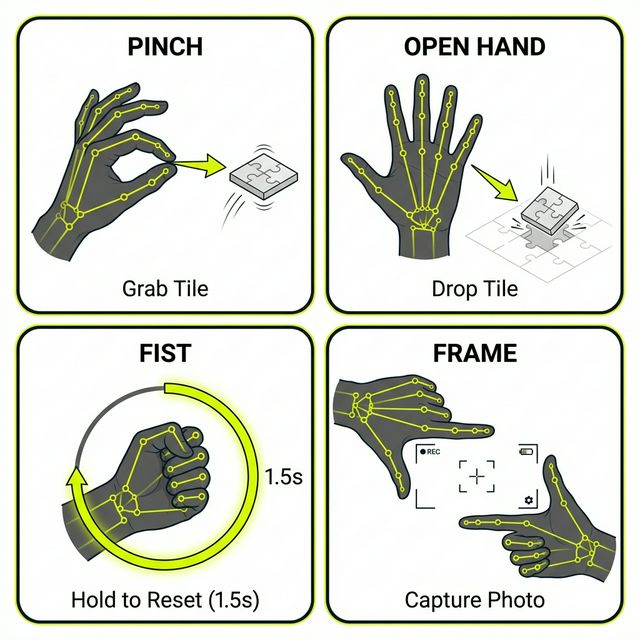
\includegraphics[width=0.7\columnwidth]{gesture_mapping.png}
\caption{Gesture-to-action mapping for the interactive puzzle game. Pinch grabs a tile, Open Hand releases it, Fist triggers a timed reset, and Frame captures a photo for the puzzle.}
\label{fig:gesture_mapping}
\end{figure}


%--- 6. DISCUSSION AND CONCLUSION ---
\section{Discussion and Conclusion}
\label{sec:conclusion}

\subsection{Summary of Findings}

\Cref{tab:bestmethod} summarizes the best-performing method for each evaluation criterion.

\begin{table}[htbp]
\centering
\caption{Best method per evaluation criterion.}
\label{tab:bestmethod}
\begin{tabular}{@{}llr@{}}
\toprule
\textbf{Criterion} & \textbf{Best Method} & \textbf{Result} \\
\midrule
Overall accuracy         & CNN / Fusion     & \SI{100.0}{\percent} \\
Skeleton-only accuracy   & MLP              & \SI{99.8}{\percent} \\
Model compactness        & MLP              & \SI{227}{\kilo\byte} \\
Generalization stability & CNN              & $\pm$\SI{0.03}{\percent} std \\
No-training deployment   & Heuristic        & \SI{170}{\byte} \\
\bottomrule
\end{tabular}
\end{table}

Three principal findings emerge from this study:

\textbf{First, data-driven methods substantially outperform hand-crafted heuristics.} The transition from the rule-based heuristic (\SI{0.99}{\percent}) to the Random Forest (\SI{94.13}{\percent}) to the MLP (\SI{99.8}{\percent}) demonstrates a clear progression where learned representations consistently outperform manually specified decision rules.

\textbf{Second, both skeleton and appearance modalities independently achieve near-perfect accuracy} on the five-class HaGRID subset. This confirms that the selected gestures are well-separated in both geometric (landmark) and visual (pixel) feature spaces. The MLP's \SI{99.8}{\percent} and CNN's \SI{100.0}{\percent} indicate that the discriminative bottleneck for this task lies not in the classification method but in the feature space definition (i.e., 5~classes are too easy for modern classifiers).

\textbf{Third, person-aware evaluation is essential for reliable performance estimation.} Group K-Fold cross-validation with person-level grouping prevents identity leakage and ensures that reported metrics reflect true generalization. The low variance across folds (MLP: $\pm$\SI{0.5}{\percent}, CNN: $\pm$\SI{0.03}{\percent}) confirms robust generalization regardless of test population composition.

\subsection{Limitations}

\begin{enumerate}
    \item \textbf{Near-ceiling accuracy:} With both modalities achieving ${\geq}$\SI{99.8}{\percent}, the fusion improvement is marginal. A more challenging gesture set (finer-grained classes, noisy environments) would better demonstrate multi-modal complementarity.
    \item \textbf{No temporal modeling:} The system classifies each frame independently, without leveraging temporal coherence across consecutive frames.
    \item \textbf{CNN latency overhead:} Adding CNN inference increases total pipeline latency. For real-time applications, the MLP alone at \SI{227}{\kilo\byte} may be preferable when latency is critical.
    \item \textbf{Dataset conditions:} HaGRID images are captured under varied but relatively controlled conditions. Performance in challenging environments (extreme lighting, motion blur, occlusion) remains to be validated.
\end{enumerate}

\subsection{Future Directions}

Future work includes: (1)~evaluating on the full 18-class HaGRID taxonomy where fusion benefits are more likely; (2)~temporal sequence modeling using LSTM or 1D-CNN architectures; (3)~attention-based fusion to learn modality-specific weighting per sample; (4)~model quantization and pruning for reduced latency on mobile devices; and (5)~user-adaptive fine-tuning to personalize gesture recognition.


%--- REFERENCES ---
\bibliographystyle{plainnat}
\begin{thebibliography}{9}

\bibitem[Kapitanov et~al.(2022)]{hagrid2022}
Kapitanov, A., Makhlyarchuk, A., and Kvanchiani, K. (2022).
\newblock {HaGRID} -- {HAnd Gesture Recognition Image Dataset}.
\newblock \emph{arXiv preprint arXiv:2206.11438}.

\bibitem[Lugaresi et~al.(2019)]{mediapipe2019}
Lugaresi, C., Tang, T., Nash, H., et~al. (2019).
\newblock {MediaPipe}: A Framework for Building Perception Pipelines.
\newblock \emph{arXiv preprint arXiv:1906.08172}.

\bibitem[Zhang et~al.(2020)]{mediapipehands2020}
Zhang, F., Bazarevsky, V., Vakunov, A., et~al. (2020).
\newblock {MediaPipe Hands}: On-device Real-time Hand Tracking.
\newblock \emph{arXiv preprint arXiv:2006.10214}.

\bibitem[Breiman(2001)]{breiman2001rf}
Breiman, L. (2001).
\newblock Random Forests.
\newblock \emph{Machine Learning}, 45(1):5--32.

\bibitem[Kingma and Ba(2014)]{kingma2014adam}
Kingma, D.~P. and Ba, J. (2014).
\newblock Adam: A Method for Stochastic Optimization.
\newblock \emph{arXiv preprint arXiv:1412.6980}.

\bibitem[Howard et~al.(2019)]{howard2019mobilenetv3}
Howard, A., Sandler, M., Chen, B., et~al. (2019).
\newblock Searching for {MobileNetV3}.
\newblock \emph{Proceedings of the IEEE International Conference on Computer Vision (ICCV)}, pp.~1314--1324.

\bibitem[Jocher et~al.(2023)]{jocher2023yolo}
Jocher, G., Chaurasia, A., and Qiu, J. (2023).
\newblock Ultralytics {YOLO} (Version 8.0.0).
\newblock \url{https://github.com/ultralytics/ultralytics}.

\bibitem[Al Farid et~al.(2022)]{alfarid2022survey}
Al Farid, F., Hashim, N., Abdullah, J., et~al. (2022).
\newblock A Structured and Methodological Review on Vision-Based Hand Gesture Recognition System.
\newblock \emph{Journal of Imaging}, 8(6):153.

\bibitem[Nguyen et~al.(2025)]{nguyen2025wheelchair}
Nguyen, T.-H., Ngo, B.-V., and Nguyen, T.-N. (2025).
\newblock Vision-Based Hand Gesture Recognition Using a {YOLOv8n} Model for the Navigation of a Smart Wheelchair.
\newblock \emph{Electronics}, 14(4):734.

\bibitem[Huda et~al.(2025)]{huda2025wheelchair}
Huda, M.~R., Ali, M.~L., and Sadi, M.~S. (2025).
\newblock Developing a real-time hand-gesture recognition technique for wheelchair control.
\newblock \emph{PLOS ONE}, 20(4):e0319996.

\end{thebibliography}

\end{document}
